\documentclass[usegraphicx,usenatbib]{mn2e}
%\documentclass[useAMS,usegraphicx,usenatbib]{mn2e}

\usepackage{verbatim}
\usepackage{color}
\usepackage[normalem]{ulem} % for striking out with \sout
\usepackage{amsmath} % for boldsymbol
\usepackage{times}
\usepackage{mathabx}
\usepackage{enumitem}

% A comment block

%\newcommand{\comment}[1]{}

% For color
\newcommand{\mpname}[1]{#1_color.eps}
\newcommand{\clraitoff}{red}
\newcommand{\lumblack}{(black)}
\newcommand{\lumblue}{(blue)}
\newcommand{\lumred}{(red)}
\newcommand{\vdisred}{(red-dashed curve)}
\newcommand{\vdisblue}{(blue-solid curve)}

% For bw
%\newcommand{\mpname}[1]{#1.eps}
%\newcommand{\clraitoff}{}
%\newcommand{\lumblack}{}
%\newcommand{\lumblue}{}
%\newcommand{\lumred}{}
%\newcommand{\vdisred}{(dashed curve)}
%\newcommand{\vdisblue}{(solid curve)}

\newcommand{\umag}{$u$}
\newcommand{\gmag}{$g$}
\newcommand{\rmag}{$r$}
\newcommand{\imag}{$i$}
\newcommand{\zmag}{$z$}
\newcommand{\gmr}{$g-r$}



\newcommand{\gammat}{$\gamma_T$}
\newcommand{\gammacross}{$\gamma_\times$}
\newcommand{\deltasig}{$\Delta \Sigma$}
\newcommand{\deltaplus}{$\Delta \Sigma_+$}
\newcommand{\deltacross}{$\Delta \Sigma_\times$}
\newcommand{\deltarho}{$\Delta \rho$}
\newcommand{\movr}{$M(<r)$}
\newcommand{\sigmacrit}{$\Sigma_{crit}$}

\newcommand{\photoz}{photo-z}
\newcommand{\photozs}{photo-zs}

\newcommand{\tlum}{$L^{tot}$}
\newcommand{\tngal}{$N_{gal}^{tot}$}

\newcommand{\lstarlim}{$0.4 L_*$}
\newcommand{\lvir}{$L_{200}$}
\newcommand{\nvir}{$N_{200}$}
\newcommand{\rvir}{$r_{200}^{gals}$}

\newcommand{\ngal}{$N_{gal}$}
\newcommand{\maxbcg}{maxBCG}
\newcommand{\numNgalBins}{12}
\newcommand{\numLumBins}{16}

\newcommand{\tngalAperture}{2$h^{-1}$ Mpc}

\newcommand{\photo}{\texttt{PHOTO}}
\newcommand{\astrop}{\texttt{ASTRO}}
\newcommand{\mt}{\texttt{MT}}
\newcommand{\spectro}{\texttt{SPECTRO}}
\newcommand{\spectroone}{\texttt{SPECTRO1d}}
\newcommand{\spectrotwo}{\texttt{SPECTRO2d}}
\newcommand{\target}{\texttt{TARGET}}

\newcommand{\lenszmax}{0.3}
\newcommand{\lenszmin}{0.05}

\newcommand{\photoversion}{\texttt{v5\_4}}

%\def\eone{e$_1$}
%\def\etwo{e$_2$}
\newcommand{\etan}{e$_+$}
\newcommand{\erad}{e$_\times$}
\newcommand{\eclass}{\texttt{ECLASS}}
\newcommand{\eclasscut}{-0.06}
\newcommand{\gmrcut}{0.7}

\newcommand{\hrs}{$^{\mathrm h}$}
\newcommand{\minutes}{$^{\mathrm m}$}

\newcommand{\ugriz}{$u, g, r, i, z$}
\newcommand{\polarization}{polarization}

\newcommand{\wgm}{$w_{gm}$}
\newcommand{\wgg}{$w_{gg}^p$}
\newcommand{\wmm}{$w_{mm}$}
\newcommand{\xigg}{$\xi_{gg}$}
\newcommand{\ximm}{$\xi_{mm}$}
\newcommand{\xigm}{$\xi_{gm}$}

\newcommand{\numspec}{127,001}
\newcommand{\numspecvlim}{10,277}
\newcommand{\numrand}{1,270,010}
\newcommand{\numspectot}{278,192}
\newcommand{\numvdis}{49,024}
%\newcommand{\numsource}{10,259,949}
% hirata: 
\newcommand{\nummask}{1,815,043}
\newcommand{\numTenMpc}{132,473}
\newcommand{\numThirtyMpc}{101,221}
\newcommand{\numsource}{27,912,891}

\newcommand{\numpairsTenMpc}{2,670,898,177}
\newcommand{\altnumpairsTenMpc}{2.7 billion}
\newcommand{\numpairsThirtyMpc}{14,818,082,122}
\newcommand{\altnumpairsThirtyMpc}{14.8 billion}



\newcommand{\xirmax}{$\xi_{gm}(R_{max})$}


\def\eps@scaling{1.0}% 

\newcommand{\sn}{$S/N$}
\newcommand{\Msn}{$(S/N)_{\textrm{matched}}$}
\newcommand{\Tsn}{$(S/N)_{\textrm{size}}$}
\newcommand{\fsn}{$(S/N)_{\textrm{flux}}$}

% stolen from the BA14 source
\newcommand{\vecg}{\mbox{\boldmath $g$}}
\newcommand{\vecD}{\mbox{\boldmath $D$}}
\newcommand{\vecQ}{\mbox{\boldmath $Q$}}
\newcommand{\matR}{\mbox{$\bf R$}}
\newcommand{\matC}{\mbox{$\bf C$}}
\newcommand{\bnabg}{ \boldsymbol{\nabla_g}}

\newcommand{\desreq}{$4\times 10^{-3}$}
\newcommand{\lsstreq}{$2\times 10^{-3}$}


\newcommand{\mnras}{MNRAS}%
\newcommand{\apj}{ApJ}%
\newcommand{\apjs}{ApJS}%
\newcommand{\aj}{AJ}%
\newcommand{\pasp}{PASP}%
\newcommand{\jcp}{J.~Chem.~Phys.}

\newcommand{\mcal}{metacalibration}
\newcommand{\Mcal}{Metacalibration}
\newcommand{\mcalR}{$R$}
\newcommand{\mcalRpsf}{$R^{p}$}
\newcommand{\mcalRpsfnoise}{$R^{p}_\eta$}
\newcommand{\mcalRo}{$R_o$}
\newcommand{\mcalRnoise}{$R_\eta$}

\newcommand{\mcalRmodel}{$R^{model}$}
\newcommand{\mcalRnoisemodel}{$R^{model}_\eta$}

\newcommand{\Aslope}{$-0.127$}
\newcommand{\Rcorr}{$-0.062$}
%\slugcomment{Last revision \today}
%\shortauthors{Sheldon}
%\shorttitle{Bayesian Shear Estimation}

\newcommand{\nsimNgal}{$10^8$}
\newcommand{\nsimNstar}{$10^7$}
\newcommand{\nsimNstarperc}{10\%}

\newcommand{\psfdist}{$(0.000,0.007) \pm 0.018$}

\title{Noise Effects in \Mcal\ Weak Lensing Shear Estimation}

\author[Erin S. Sheldon]{Erin S. Sheldon\thanks{E-mail: erin.sheldon@gmail.com}\\
Brookhaven National Laboratory, Bldg 510, Upton, New York 11973}

\begin{document}

\maketitle

\begin{abstract}

I implement corrections for sheared correlated noise effects in \mcal, and
explore the effects of stellar contamination and masking.   

\end{abstract}


\begin{keywords}                                                                    
    cosmology: observations,
    gravitational lensing: weak,
    dark energy
\end{keywords} 

\section{Introduction} \label{sec:intro}

\section{\Mcal} \label{sec:algo}

Suppose we have a biased shear estimator $E$.  We can expand this estimator
in a Taylor series around the true shear
\begin{align}
    E(\gamma) &= E(\gamma=0) + \gamma ~ \frac{ \partial E }{ \partial \gamma }\bigg|_{\gamma=0}  + ... \nonumber \\
      & \approx  \gamma ~ \frac{ \partial E }{ \partial \gamma } \bigg|_{\gamma=0}  \\
      & \equiv  \gamma ~ \mbox{\mcalR} \nonumber
\end{align}
where $\gamma$ is denotes the true gravitational shear.  We call \mcalR\
the shear response.

The essence of \mcal\ \citep{HuffMcal} is to estimate the shear response
\mcalR\ for a shear estimator $E$ directly from image data.  This is
accomplished using a numerical derivative.  The original image $I$ is
de-convolved from the point spread function (PSF), sheared, and re-convolved
with a slightly larger PSF.  This \mcal\ process is repeated for a
positive and negative shear, which can be used to form a central derivative.
We can represent this as a series of operations on the observed image $I$:
\begin{equation}
    I(\gamma) = I \Asterisk P^{-1} \oplus \gamma \Asterisk P_{d}
\end{equation}
where $\Asterisk$ represents convolution, $\oplus$ represents shearing,
and $P$ represents the point spread function.  De-convolution
is represented as ``inverse``, $P^{-1}$.  The slightly larger PSF, or
dilated PSF, is represented by $P_{d}$.

To form the central derivative we shear by a small positive and negative
amount $\gamma$
\begin{equation} \label{eq:Rnum}
    R = \frac{E(+\gamma) - E(-\gamma)}{2 \gamma}.
\end{equation}
The shear estimator can also be derived from the re-convolved
images
\begin{equation} \label{eq:estimator}
    E = \frac{E(+\gamma) + E(-\gamma)}{2}.
\end{equation}

For a constant shear, the response and shear estimators can be averaged
separately and combined to recover the mean shear:
\begin{equation}
    \gamma = \frac{ \langle E \rangle }{\langle \mbox{\mcalR} \rangle}.
\end{equation}
In \cite{HuffMcal} a more sophisticated inference was used, in order to deal
with the relatively large variance in \mcalR\ associated with the particular
estimator used therein.

Another correction can be derived for errors in the correction for 
PSF anisotropy.  This correction involves shearing the PSF rather
than the galaxy:
\begin{equation}
    \mbox{\mcalRpsf} = \frac{E(+\gamma^{p}) - E(-\gamma^{p})}{2 \gamma^{p}},
\end{equation}
where $\gamma^{p}$ is a shear applied to the PSF.  This
term adds to the estimator $E$, multiplied by the PSF shape
\begin{equation}
    E = \mbox{\mcalR} \gamma + \mbox{\mcalRpsf} e^{p} 
\end{equation}
This term can be subtracted to approximately correct for additive PSF errors:
\begin{equation}
    \gamma = \frac{ \langle E \rangle - \langle \mbox{\mcalRpsf} e^{p} \rangle }{\langle \mbox{\mcalR} \rangle}.
\end{equation}
In practice we calculate mean responses, factoring out the response term:
\begin{equation}
    \gamma = \frac{ \langle E \rangle - 
            \langle \mbox{\mcalRpsf}\rangle \langle e^{p} \rangle }{\langle \mbox{\mcalR} \rangle}.
\end{equation}


\section{Contamination of the Response by Correlated Noise} \label{sec:contam}

In the presence of noise, the observed image can be written $I_o=I+\eta$, where $\eta$
is the ``noise image``.  The \mcal\ sheared images $I_o(\gamma)$ will contain
contributions from de-convolved, sheared and re-convolved noise:
\begin{align}
    I_{o}(\gamma) &= (I + \eta) \Asterisk P^{-1} \oplus \gamma \Asterisk P_{d} \nonumber \\
    &= I(\gamma) + \eta(\gamma).
\end{align}
The de-convolution correlates the noise
across the image.  This correlated noise is sheared, and then re-convolved by
the dilated PSF, producing the sheared correlated noise image $\eta(\gamma)$.

We expect the sheared correlated noise to partly cancel in the estimator in
equation \ref{eq:estimator}, because the effect is averaged over both positive
and negative shears. This quantity is further averaged over many galaxies.

However, the sheared correlated noise term will not cancel when calculating the
response, which is the difference of positive and negative shears.  This
remainder is amplified due to division by $2 \gamma$ to form the central
derivative.  We thus expect the observed response \mcalRo\ to be contaminated
by the response of the correlated, sheared noise \mcalRnoise\
\begin{equation}
    \mbox{\mcalRo}  =  R + \mbox{\mcalRnoise}
\end{equation}

A correction is also required for the PSF response term \mcalRpsf.  We find
this correction is similar in magnitude to the correction for \mcalR, although
it is somewhat suppressed in the final estimator due to multiplication by $e^p$.


\begin{comment}
\subsection{Expected Level of Contamination}

I think the following is not correct.

The correlated noise is produced by de-convolving and re-convolving by the psf,
so it may be correlated with the PSF ellipticity at some level.  Let's assume
the induced ellipticity is $f \times e^{PSF}$ in the absence of shearing, with
$f$ small.  We expect this to cancel in the response calculation, due to the
subtraction, but add to the estimator $E$.  This should, however, be
partly dealt with by subtracting $R^{PSF}$ (see below).

If we introduce shearing, then the sheared noise will cancel in the estimator
$E$ but not the response.

This sheared part of the correlated noise is suppressed by a factor of
$\gamma$, but in forming the derivative another factor of $1/\gamma$ is
applied.  Thus we expect the overall contamination $R_\eta$ to be of
the order $f \times e^{PSF}$.

\end{comment}

\section{Correction for Sheared, Correlated Noise} \label{sec:corr}

For shear estimators based on raw moments, without any form of iteration or
fitting, it would be sufficient to simply measure the moments of example
sheared correlated noise fields and subtract the mean response from the
responses measured on the real images.  Multiple realizations can be generated
for each galaxy to increase precision.

For non-linear fitting, we propose three methods to correct for the effects of
the sheared, correlated noise on the measured response.  The first is based on
de-trending the effects of correlated noise, which we find accurate and well
motivated theoretically.  We discuss this method in detail in \S
\ref{sec:detrend}.  The second is based on adding a sheared, correlated noise
field that has been sheared with the opposite sign.  The third is based on
simulating the effect on modeled images.  We discuss methods two and three in
the appendix.


\subsection{Detrending the Correlated Noise Bias} \label{sec:detrend}

The bias in \mcalR\ due to correlated noise should scale with the 
noise correlation function, and thus the square of the noise level
in the image $n^2$ \citep{HirataCorrNoise}.  The observed \mcalRo\
is given by
\begin{align} \label{eq:scaling}
    \mbox{\mcalRo} &= R + \mbox{\mcalRnoise}  \nonumber \\
                   &= R + A n^2
\end{align}
We can add a small amount of noise to the image
such that $n \rightarrow n + \Delta n$. We then run the new image
through the \mcal\ process, and measure $R^{\mathrm{before}}$.  We can also
add identical noise {\em after} the original image  has been run through \mcal, and
measure $R^{\mathrm{after}}$.  The response when adding noise before
\mcal\ is given by
\begin{align}\label{eq:Rbefore}
    R_o^{\mathrm{before}} &= R + A (n + \Delta n)^2 \nonumber \\
       &\simeq R + A n^2 + 2 A n \Delta n
\end{align}
%&\simeq R + A n^2 + \frac{\partial (An^2)}{\partial n} \Delta n + ... \nonumber \\
where we have dropped terms of order $(\Delta n)^2$ and higher.  In equation
\ref{eq:Rbefore}, \mcalR\ is the response at noise $n+\Delta n$ in the absence
of correlated noise.  The response when adding noise after \mcal\ does
not suffer any additional bias due to correlated noise:
\begin{align}
    R_o^{\mathrm{after}} &= R + A n^2.
\end{align}
The difference between these responses is then 
\begin{align}
    \Delta R &\equiv R_o^{\mathrm{before}} - R_o^{\mathrm{after}}  \nonumber \\
             &\simeq 2 A n \Delta n.
\end{align}

The procedure we propose is 
\begin{enumerate}
    \item Calculate $\Delta R$ for a series of noise offsets $\Delta n$.
    \item Average $\Delta R$ over all objects
    \item Perform a linear fit to $\Delta R$ vs. $2 n \Delta n$ to find the 
        coefficient $A$.
    \item Apply a mean correction for correlated noise given by
        \begin{align}
            \mbox{\mcalRnoise} & \simeq A n^2.
        \end{align}
        with a similar correction for \mcalRpsf.
\end{enumerate}
If the noise varies between observations, we can apply a 
correction based on the mean variance $A
\langle n^2 \rangle$.


\section{Image Simulations}

We apply the de-trending correction scheme to a set of image simulations.  The
first simulations make use of parametric models, and are designed to be similar
to that used in \citet{bfd2015}.  The galaxies are bulge+disk models with both
components having the same ellipticity and half light radius, drawn from a
log-normal distribution centered at 2.0 pixels, with scatter of 0.5 pixels.
The bulges are offset uniformly up to a scale length.  The ellipticities were
drawn from the simple model presented in \cite{ba14}, with $\sigma=0.2$.  The
PSF is an elliptical Moffat profile (ref?), with $r_{50} = 1.5$ pixels. The PSF
ellipticity was drawn from a double Gaussian with width 0.018, designed to
match that measured for the Dark Energy Survey \citep{DESSVShear}. The mean in
$e_2$ was set to 0.007, also matching DES, but the mean in $e_1$ was set to 0.0
as a baseline reference.  The S/N distribution matches real DES data, with $S/N
\gtrapprox 10$.  Galaxies were sheared with 300 different randomly chosen
shears, ranging from 0.01 to 0.08 in amplitude.

\begin{table*}
    \centering
    \caption{Description of the image simulations.}
    \begin{tabular}{ | c | c | c | c | c | c | c | c | c |}
        Sim        & Galaxy Model & PSF Model & Gal Shape $\sigma$ & PSF Shape  & \# Galaxies & \# Stars    & Masking & Selection  \\
        \hline
        BD         & Bulge+Disk   & Moffat    & 0.2                & \psfdist & \nsimNgal   & None        & None    & None  \\
        BDStar     & Bulge+Disk   & Moffat    & 0.2                & \psfdist & \nsimNgal   & \nsimNstar  & None    & None  \\
        BDStarMask & Bulge+Disk   & Moffat    & 0.2                & \psfdist & \nsimNgal   & \nsimNstar  & DES     & None  \\
        BDStarMaskSN10 & Bulge+Disk   & Moffat    & 0.2            & \psfdist & \nsimNgal   & \nsimNstar  & DES     & $(S/N) > 10$ \\
        BDStarMaskSN15 & Bulge+Disk   & Moffat    & 0.2            & \psfdist & \nsimNgal   & \nsimNstar  & DES     & $(S/N) > 15$ \\
        BDStarMaskSN20 & Bulge+Disk   & Moffat    & 0.2            & \psfdist & \nsimNgal   & \nsimNstar  & DES     & $(S/N) > 20$ \\
    \end{tabular}
\end{table*}

Describe egret sims here.

The images were fit with a single Gaussian galaxy model and Gaussian PSF model.
Naively using these simple galaxy and PSF model results in a large model bias,
and large uncorrected PSF anisotropy.

A maximum likelihood fit was used, with smooth priors on all parameters to
produce a stable fit.  These priors were not tuned to the true galaxy
parameters; priors on flux and size were deliberately wider than truth by 20\%,
and that on ellipticity used $\sigma=0.3$ instead of the true $0.2$.  We
furthermore expect large {\em ordinary} noise bias at these low S/N levels.

\section{Results} \label{sec:detrendsim}

\begin{table*}
    \centering
    \caption{\mcal\ results for each image simulation.}
    \begin{tabular}{ | c | c | c | c | c | c | c | c | c | c | c | c |}
        Sim & $m_1 \times 10^4$ & $m_2 \times 10^4 $ & $c_1 \times 10^5$ & $c_2 \times 10^5$ \\
        \hline
        BD          & $6.1 \pm 6.1$ & $3.1 \pm 6.4$ & $-3.1 \pm 2.1$ & $-2.2 \pm 2.1$   \\
        BDStar      & $6.1 \pm 6.1$ & $3.1 \pm 6.4$ & $-3.1 \pm 2.1$ & $-2.2 \pm 2.1$   \\
        BDStarMask  & $6.1 \pm 6.1$ & $3.1 \pm 6.4$ & $-3.1 \pm 2.1$ & $-2.2 \pm 2.1$   \\
    \end{tabular}
\end{table*}


The measurement of $\Delta R$ vs $2 n \Delta n$ is shown in figure
\ref{fig:detrend}.  The trend is well-fit by a linear model, as expected, with
a slope $A \simeq $\Aslope, implying a correction $A n^2 \simeq$ \Rcorr\ for this
simulation.

\begin{figure}
    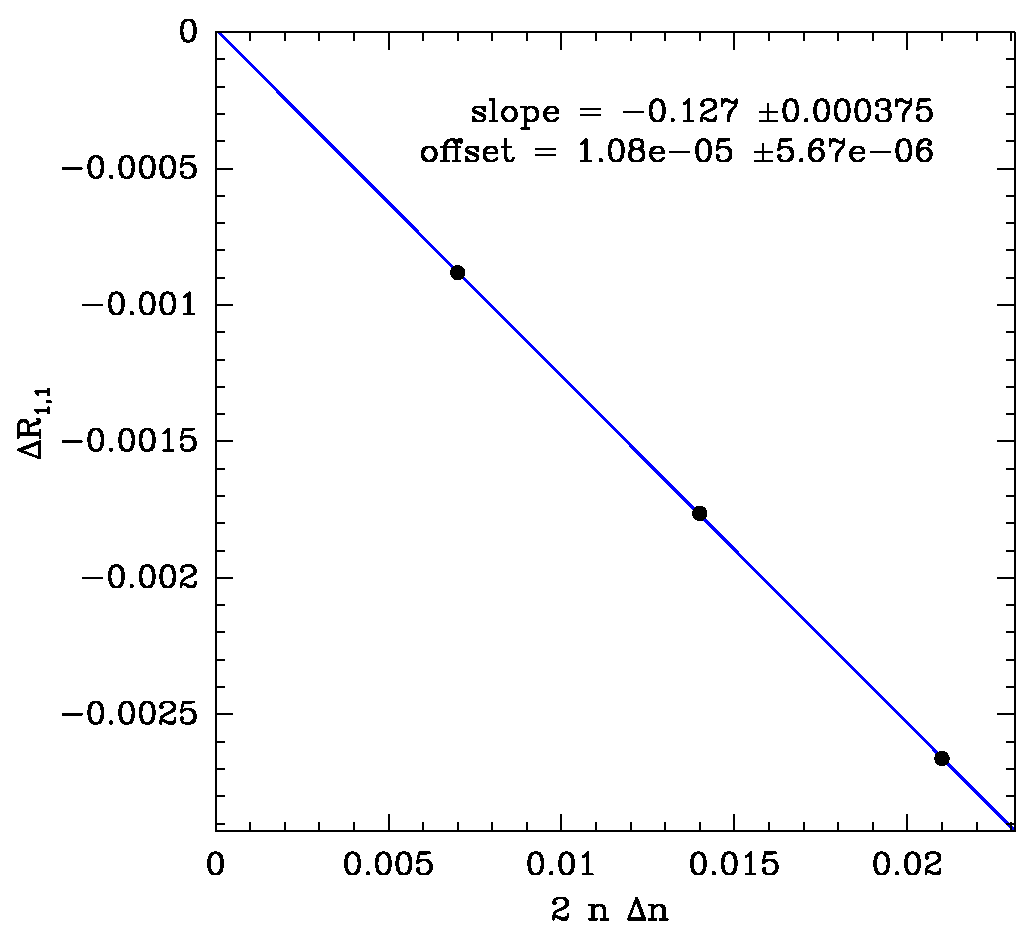
\includegraphics[scale=0.45]{run-bd13mcal-dt02-Rnoise-detrend-R11.eps}

    \caption{Trend of $\Delta R_{1,1}$ with $2 n \Delta n$, where $n$ is the
    original noise level and $\Delta n$ is the additional noise added.  The
trend is linear  as predicted.}

\label{fig:detrend}
\end{figure}

Applying these corrections to $R$, we recover the shear within the
measurement error
\begin{align} \label{eq:detrendres}
    m_1 &= ( 6.1 \pm 6.1) \times 10^{-4} \nonumber \\
    m_2 &= ( 3.1 \pm 6.4) \times 10^{-4} \nonumber \\
    c_1 &= (-3.1 \pm 2.1) \times 10^{-5} \nonumber \\
    c_2 &= (-2.2 \pm 2.1) \times 10^{-5}. \nonumber
\end{align}
Without correction, the multiplicative bias $m$ is $\simeq$ 10\%
for these simulations.

\subsection{Stellar Contamination} \label{sec:stars}

We included an additional \nsimNstar\ stellar objects, drawn simply as a
PSF with noise added.

\subsection{Masking Effects} \label{sec:masking}

%\subsection{Selection Effects} \label{sec:selection}

\subsection{Using a Random Subset To Calculate Detrending Corrections}

The detrending parameters are precisely measured relative to the shear itself.
Here we explore the precision of the recovered shear using subsets of
the objects to measure detrending.  In Table \ref{tab:subsets} we 
have shown the
shear recovery parameters for various subset sizes, for the same simulation
described in \S \ref{sec:detrendsim}

\begin{table}[h] 
    \centering
    \caption{Additional variance in the recovered shear using the
        detrending method, using different sized subsets to
        estimate the correctios.  Values are obtained
        from 100 bootstrap samples. \label{tab:subsets}}
    \begin{tabular}{| c | c |}
        Subset Size & Extra Error \\
        \hline
        1\% & 4.4\% \\
        5\% & 0.8\% \\
        10\% & 0.3\% \\
    \end{tabular}
\end{table}
%        1\% & 30\% \\
%        5\% & 13\% \\
%        10\% & 8\% \\


To calculate these numbers we have assumed the extra uncertainty is added
quadratically with the measured uncertainty; e.g for the first row, we have
added approximately 30\% quadratically with the measured uncertainty, resulting
in a net increase of 4.4\%.

It is important to use a truly random subset of the population, including a
fair sample of stars contaminate the sample, and a representative level of
pixel level masking.  If a particular aggregate shear measurement involves a
selection, this selection must also be applied to the random subset.

\section{Cancellation in Ring Configurations}

This bias was not seen by \cite{HuffMcal} using the GREAT3 simulations
\citep{great3}.

The only substantial difference between the GREAT3 sims and our sims is that
GREAT3 galaxies were generated in a ``ring configuration''.  The simulation
included two identical images of each galaxy, rotated by 90 degrees with
respect to a one another, in order to cancel shape noise.  In this configuration,
the correlated noise also appears to cancel at some level.

\appendix

\section{Additional Correction Methods}

\subsubsection{Adding a Sheared, Correlated Random Noise Field}

In this method, we generate example random noise fields $\tilde{\eta}$, sheared
with the opposite sign of those used in the \mcal\ procedure:
\begin{equation}
    \tilde{\eta}(-\gamma) = \tilde{\eta} \Asterisk P^{-1} \oplus (-\gamma) \Asterisk P_{d}.
\end{equation}
This noise image can then be added to the $I(\gamma)_o$ images to
statistically remove the effects of sheared, correlated noise:
\begin{equation}
    \tilde{I}(\gamma) = I_o(\gamma) + \tilde{\eta}(-\gamma),
\end{equation}
where $\tilde{I}(\gamma)$ is an approximation for the desired image
$I(\gamma)$.    These $\tilde{I}(\gamma)$
can be used to measure the correct \mcal\ for a large population.
It is important that the random noise field be added after
the \mcal\ procedures have been applied, not before.

This procedure increases the noise by a factor of $\sqrt 2$.  Thus, both the
response and estimator should be measured on the $\tilde{I}(\gamma)$ images, so
that the response is representative of the correct noise level.  To reduce the
noise in the fits, multiple random fields can be generated and added to the
original image, and these can all then be fit simultaneously.  This will
improve the precision of the fit, at the cost of increased computation time.


\subsubsection{Simulating Models}

In this method, we generate model images with the right noise level for a
given galaxy, and then measure the response of the noise due to the
convolutions and shears used in \mcal.  We then subtract the mean sheared noise
response from the mean measured response, averaged over some set of galaxy
images. The process is as follows:
\begin{enumerate}[label=\arabic*.]

    \item Measure the response without correlated noise
    
        \begin{enumerate}[label*=\arabic*.]
            \item Render the best fit model, including convolution by the point-spread
                function

            \item Perform the \mcal\ image processing steps, without noise added.

            \item Add an appropriate amount of noise to all images, using the
                same noise pattern $I_\eta$ for every image.

            \item Measure the response for this model \mcalRmodel.
        \end{enumerate}

    \item Measure the response with correlated noise
    
        \begin{enumerate}[label*=\arabic*.]
            \item Render the best fit model, including convolution by the point-spread
                function

            \item Add an appropriate noise pattern $I_\eta$ to the image, the
                same pattern used for measuring the response without correlated
                noise.

            \item Perform the \mcal\ image processing steps on this noisy
                image.

            \item Measure the response for this model \mcalRnoisemodel.

        \end{enumerate}

    \item Subtract the correlated noise response

\end{enumerate}

The measurement with correlated noise will be the sum of the response
without correlated noise plus the response of the correlated noise field
\begin{equation}
    \mbox{\mcalRnoisemodel} = \mbox{\mcalRmodel} + \mbox{\mcalRnoise}
\end{equation}
This measurement is quite noisy for a single galaxy, but we
can estimate the mean correlated noise response for an ensemble
of galaxies
\begin{equation}
    \langle \mbox{\mcalRnoise} \rangle = \langle \mbox{\mcalRnoisemodel} \rangle - \langle \mbox{\mcalRmodel} \rangle.
\end{equation}
Each entry used in this average corresponds to the best fit model
and noise properties for a galaxy in the sample.

The response \mcalRnoise\ can be subtracted to recover an estimate of the mean
response without correlated noise
\begin{equation}
    \langle \mbox{\mcalR} \rangle = \langle \mbox{\mcalRo} \rangle - \langle \mbox{\mcalRnoise} \rangle.
\end{equation}
These responses will be noisier than the original images, due to the
independent noise in both \mcalRo\ and \mcalRnoise.  To increase
precision, the procedure can be repeated for different noise fields
and averaged, at the cost of increased computation time.


\bibliographystyle{mn2e}
% Bib database
\bibliography{apj-jour,astroref}

\end{document}

